%empezar con (por arriba) qué es sintesis y para que sirve. X ej para situaciones que no se puede programar o adaptar programas en el momento (vuelo de aviones?). (verificación de software?)

El ser humano siempre buscó la manera de automatizar las tareas pesadas o tediosas, la ciencia de la computación surgió en parte a causa de ello pero ¿Podríamos automatizar aún más? 
Hacer que una computadora ``se programe'' a sí misma dado un problema a resolver es en cierta medida una utopía, sin embargo hay muchas ramas de la computación que atacan ésta idea. Ya sea Machine Learning, Inteligencia Artificial ó, en el caso del presente trabajo, Síntesis Automática de Controladores.

\textit{Síntesis} porque no es un humano quien desarrolla manualmente el código \textit{solución} del problema sino que se le brinda a un programa las reglas y objetivos a cumplir, dejando ``a criterio del mismo'' el cómo hacerlo. Lo que devuelve el programa es una \textit{estrategia} que garantiza ganar (si existe forma, caso contrario avisa la inexistencia de solución), a ésta estrategia se la conoce con el nombre de \textit{Controlador}.

Un ejemplo de aplicación es controlar aviones para demarcar incendios forestales \textcolor{red}{[REF]}, donde a veces incluso es necesario que el programa pueda adaptarse en medio de su ejecución. %TODO explicamos algo más?

%Existen varias ramas que investigan esto de formas similares. Una mini explicación de cada una?
El problema de síntesis fue estudiado dentro de distintas áreas como: Control de Eventos Discretos \textcolor{red}{[REFS]}, Síntesis Reactiva \textcolor{red}{[REFS]} y Planning automático \textcolor{red}{[REFS]}. %TODO explicar algo de cada una? (poco)
Si bien este trabajo desarrolla resultados nuevos combinando enfoques de las tres áreas, nos basamos principalmente en Control de Eventos Discretos (Discrete Event Control ó DEC).

%DEC modela como un autómata (estados del programa donde uno se mueve dirigido con eventos, ver caso de estudio) donde busca estados ganadores?
 En DEC el problema es modelado utilizando autómatas finitos, también conocidos como máquinas de estados finitos. 
Un autómata finito, está conformado por estados y transiciones entre éstos estados. Podemos pensar los estados como puntos y las transiciones como flechas de un sólo sentido que los unen. Se los llama estados ya que representan un momento particular en el objeto que se quiere modelar, por ejemplo en el caso del avión un estado podría ser ``aterrizado'' y otro ``en vuelo''. Las transiciones en nuestro caso son vistas como acciones, algunas las podemos controlar y otras están fuera de nuestro alcance; volviendo al ejemplo del avión una acción controlable podría ser ``encender el motor'' y una no controlable sería ``quedarse sin combustible''.

Además existen estados distinguidos dentro del autómata: el inicial (estado en cuál empezamos) y los estados objetivos (a los cuáles se quiere llegar). En nuestro caso a éstos últimos los llamamos \textit{estados marcados} y no sólo queremos alcanzarlos sino ser capaces de hacerlo infinitas veces y se manera segura. Segura en el sentido de siempre tener una secuencia de acciones para llegar, ¡no podemos quedarnos sin transiciones ni usarlas en el sentido contrario!

Por último, modelar un sistema complejo utilizando un sólo autómata puede ser complicado y hasta imposible. Es por esto que se suele modelar sus partes como autómatas y componerlos para formar el sistema. La composición debe respetar ciertas reglas y al finalizar, un estado del sistema representaría un conjunto de estados de los componentes. %TODO explicamos las reglas? ponemos un ejemplo de a qué nos referimos?

%tradicionalmente se compone todo y se explora fácil. Nosotros exploramos on-the-fly. Como se ve en caso de estudio, el tamaño de la planta crece muy rápido, por eso la técnica todavía no es popular para problemas grandes. Eso lo tratamos de mitigar con on-the-fly
Tradicionalmente se toman estos autómatas componentes y se realiza la composición, obteniendo el autómata del sistema que luego será analizado por el programa para obtener el controlador. El problema es que en ciertos casos la cantidad de estados y transiciones resultantes del sistema es demasiado grande, haciendo imposible su análisis y en ocasiones hasta es imposible terminar de componer.

Es en éste contexto que surge el enfoque de la exploración on-the-fly o ``en el mientras''. La idea es tratar de sacar conclusiones mientras se va calculando la composición para, de ésta manera, evitar en lo posible construir todo el sistema. Para evidenciar la dificultad de la cuál se está hablando presentaremos un caso de estudio, sus componentes y el sistema resultante de la composición.


\section{Caso de estudio}\label{chpt:casoAviones}
A continuación se presenta un ejemplo para comprender el problema a resolver. Se trata de una versión simplificada del problema $Travel Agency$ utilizado en el capítulo \ref{chpt:performance} para medir la performance del algoritmo.

Se desea armar una agencia de venta online de paquetes vacacionales que reservará de forma automática una variedad de servicios (alquiler de auto, hotel, pasaje de avión, etc.) asegurando que no se perderá nada de dinero a menos que se reserve el paquete completo. Es decir, no se quiere perder dinero por la reserva del hotel si no va a ser posible comprar un pasaje de avión.

Para cada servicio que se desea sub-contratar se consulta si ese servicio está disponible. En caso de confirmar la disponibilidad, se espera a confirmar el resto para comprar todos al  mismo tiemmpo. En caso de que algún otro servicio no esté dispoinble, se cancela la compra y se vuelve al estado inicial, lo cual no implica un gasto.

El problema puede escalar de forma muy rápida si se incrementa la cantidad de servicios a contratar o la cantidad de pasos para reservar cada servicio (como se verá en la sección~\ref{chpt:performance}).

Mostramos en la figura~\ref{fig:N1} un LTS (Labeled transition system) para cada uno de los componentes descriptos y el LTS compuesto para el caso en el que se sub-contrata un solo servicio.

\begin{figure}[htb]
	\begin{center}
		\makebox[\linewidth][c]{%
			\begin{subfigure}[t]{.5\textwidth}
				\centering
				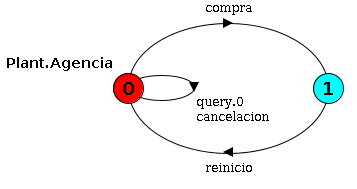
\includegraphics[width=\linewidth]{figures/ejemploServicios/agencia.png}  
				\caption{agencia}
				\label{fig:agencia}
			\end{subfigure}
			\begin{subfigure}[t]{.5\textwidth}
				\centering
				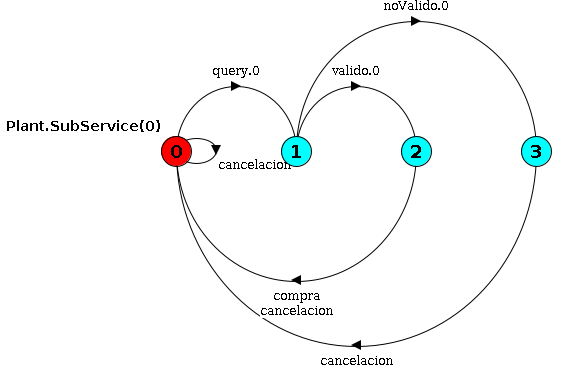
\includegraphics[width=\linewidth]{figures/ejemploServicios/subServicio.png}  
				\caption{un sub servicio}
				\label{fig:subserv}
			\end{subfigure}
		}
		\makebox[\linewidth][c]{%
			\begin{subfigure}[t]{.5\textwidth}
				\centering
				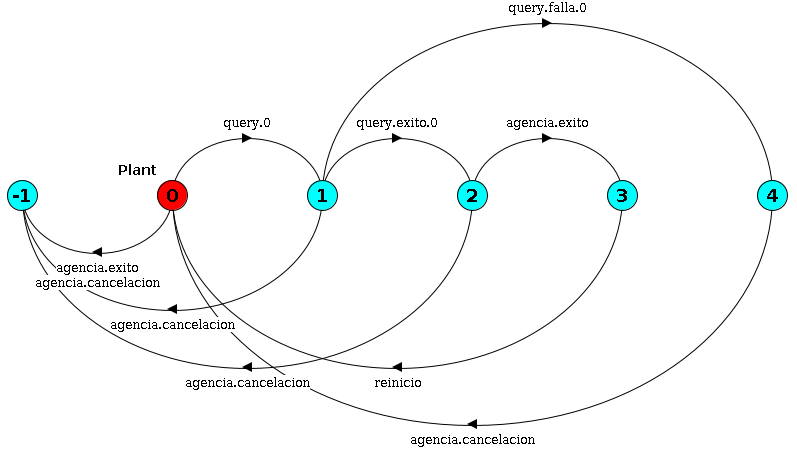
\includegraphics[width=\linewidth]{figures/ejemploServicios/N1Planta.png}  
				\caption{Planta compuesta}
				\label{fig:N1Planta}
			\end{subfigure}
			\begin{subfigure}[t]{.5\textwidth}
				\centering
				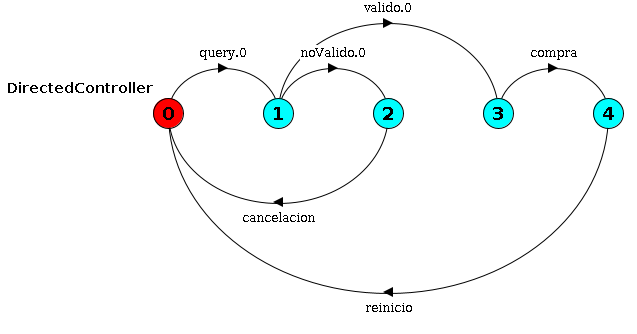
\includegraphics[width=\linewidth]{figures/ejemploServicios/N1Controlador.png}  
				\caption{Controlador resultante}
				\label{fig:controladorN1}
			\end{subfigure}
		}
		\caption{Caso con un solo sub-sevicio}
		\label{fig:N1}
	\end{center}
\end{figure}

\begin{figure}[htb]
	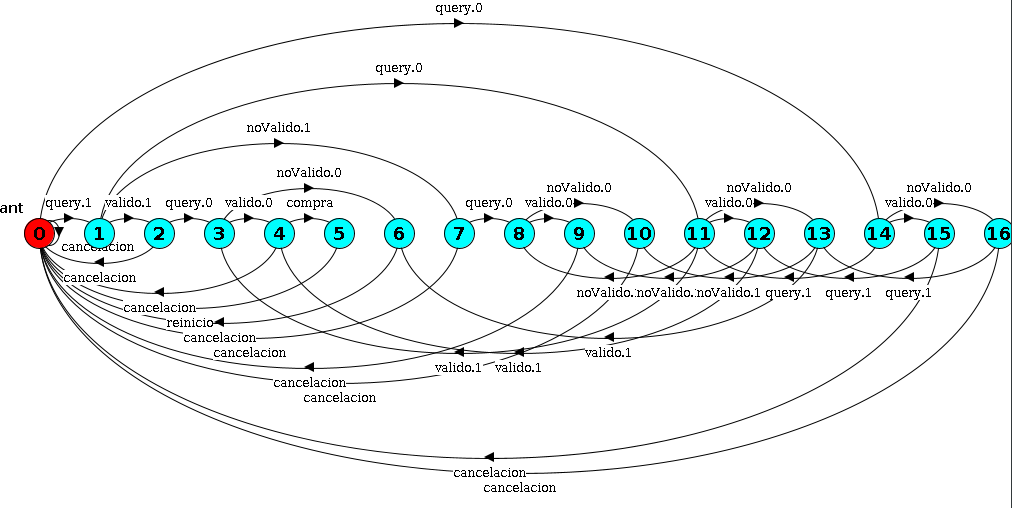
\includegraphics[width=\linewidth]{figures/ejemploServicios/N2Planta.png}  
	\caption{Planta compuesta con 2 sub-servicios}
	\label{fig:N2}
\end{figure}

En el ejemplo, la figura \ref{fig:agencia} representa a la agencia, que comienza en el estado inicial (0), y lo que quiere es confirmar la compra. Mientras siga consultando la disponibilidad del servicio con \textit{query.0} y cancelando la compra, su estado no cambia. 

Ahora, el componente del subservicio (figura \ref{fig:subserv}) también tiene el evento \textit{compra}, pero antes de poder confirmarse la compra del subservicio debe previamente haber recibido la consulta (\textit{query.0}) y confirmado su disponibilidad tomando el evento \textit{valido.0}. En caso de no estar disponible (\textit{noValido.0}) solo permite la cancelación de la compra, yendo del estado 3 al 0.

Recordemos que queremos representar un sistema complejo con interacción de múltiples componentes. Esta sincronización se ve reflejada en la figura \ref{fig:N1Planta}, que muestra la planta que representa al sistema con los dos componentes. 

Finalmente, \ref{fig:controladorN1} muestra un posible controlador para este problema. Destacamos que el evento controlable \textit{cancelacion}, no está habilitado si se confirmó la validez del subservicio, y el controlador es de hecho un director (definido en la sección \ref{chpt:director}). 

Puede verse que para el caso de solo un sub-servicio que debe ser contratado el problema es manejable. Los modelos gráficos de la planta y el controlador, generados automáticamente por MTSA\footnote{Modal Transition System Analyser, \href{https://bitbucket.org/lnahabedian/mtsa/src/master/^}{https://bitbucket.org/lnahabedian/mtsa/src/master/}} se comprenden con un vistazo. Ya el caso con $N=2$ (fig~\ref{fig:N2}) si bien puede generarse una representación gráfica, requiere un trabajo considerable para comprender qué estado del problema representa cada estado del modelo. Simplemente aumentando a $N=5$ ya la planta compuesta cuenta con 1025 estados y 4085 transiciones, imposibilitando mostrarlo en una figura. 

Los algoritmos tradicionales necesitan construir el sistema compuesto entero antes de empezar, es por ésta explosión de estados y transiciones que resulta muy costoso (aveces imposible), por ende los algoritmos de punto fijo pueden manejar hasta cierto tamaño de problemas. En el caso de on-the-fly al ser una exploración dirigida construye sólo lo necesario, sacando conclusiones en función de la información obtenida; en el peor caso puede contruir todo (si es que esto es posible).

\section{Estructura de los capítulos}

A continuación presentamos los antecedentes, definiciones necesarias y un algoritmo tradicional monolítico; ésto puede encontrarse en el capítulo \ref{chpt:background}.

En el capítulo \ref{chpt:on-the-fly}, presentamos la idea básica de exploración on-the-fly junto con una descripción de nuestro enfoque en particular, como forma introductoria al siguiente capítulo.

Ya con las intuiciones del algoritmo introducidas, el capítulo \ref{chpt:dcs} muestra nuestra propuesta de algoritmo en detalle, con el pseudocódigo, demostración corrección y completitud para el mismo y análisis de la complejidad computacional de su peor caso.

Luego exponemos detalles sobre la implementación en el capítulo \ref{chpt:implementation}, MTSA, heurísticas diseñadas para testeo y detalles sobre la batería de test, desarrollada utilizando TDD (Test Driven Development).

Como paso final en el capítulo \ref{chpt:performance} presentamos el benchmark utilizado y resultados de performance; tanto versus la versión anterior de DCS como versus otros algoritmos del estado del arte.

Finalmente, listamos las conclusiones y aportes del trabajo presentado.









